%%%%%%%%%%%%%%%%%%%%%%%%%%%%%%%%%%%%%%%%%%%%%%%%%%%%%%%%%%%%%%%%%%%%%%%%%%%%%%%%
%2345678901234567890123456789012345678901234567890123456789012345678901234567890
%        1         2         3         4         5         6         7         8

\documentclass[letterpaper, 10 pt, conference]{ieeeconf}  % Comment this line out if you need a4paper

%\documentclass[a4paper, 10pt, conference]{ieeeconf}      % Use this line for a4 paper

\IEEEoverridecommandlockouts                              % This command is only needed if 
                                                          % you want to use the \thanks command

\overrideIEEEmargins                                      % Needed to meet printer requirements.

% See the \addtolength command later in the file to balance the column lengths
% on the last page of the document

% The following packages can be found on http:\\www.ctan.org
%\usepackage{graphics} % for pdf, bitmapped graphics files
%\usepackage{epsfig} % for postscript graphics files
%\usepackage{mathptmx} % assumes new font selection scheme installed
%\usepackage{times} % assumes new font selection scheme installed
%\usepackage{amsmath} % assumes amsmath package installed
%\usepackage{amssymb}  % assumes amsmath package installed
\usepackage{amsmath}
\usepackage{amsfonts}
\usepackage{amssymb}
\usepackage{hyperref}
\usepackage[colorinlistoftodos]{todonotes}

\title{\LARGE \bf
Preparation of Papers for IEEE Sponsored Conferences \& Symposia*
}


\author{Benjamin Reinhardt$^{1}$ % and Bernard D. Researcher$^{2}$% <-this % stops a space
\thanks{*This work was supported by a NSTRF Grant}% <-this % stops a space
%\thanks{$^{1}$Albert Author is with Faculty of Electrical Engineering, Mathematics and Computer Science,
%        University of Twente, 7500 AE Enschede, The Netherlands
%        {\tt\small albert.author@papercept.net}}%
%\thanks{$^{2}$Bernard D. Researcheris with the Department of Electrical Engineering, Wright State University,
%        Dayton, OH 45435, USA
%        {\tt\small b.d.researcher@ieee.org}}%
}


\begin{document}



\maketitle
\thispagestyle{empty}
\pagestyle{empty}


%%%%%%%%%%%%%%%%%%%%%%%%%%%%%%%%%%%%%%%%%%%%%%%%%%%%%%%%%%%%%%%%%%%%%%%%%%%%%%%%
\begin{abstract}

Can you move along a surface in space without propellant or physical contact? On-orbit servicing requires a robot to operate in close proximity to the surface of a target spacecraft in order to inspect, refuel, or repair it.  Robotic operation at such small distances is difficult in space because spacecraft are fragile and often have poorly known dynamics that are never damped out by the environment. Current actuators for locomotion and grasping during on-orbit servicing require physical contact with the target, propellant, or cooperation from the target.  
%
This paper presents an new actuator - the induction coupler - that generates eddy-current forces between a robotic orbital inspector and the conductive exterior of its target. These forces allow the inspector to crawl along the surface of a target while maintaining a safety gap. Sets of induction couplers can exert control forces and torques in all six rigid-body degrees of freedom by strategically repelling and shearing across the surface of the target. Spinning arrays of permanent magnets produce shearing eddy-current forces and current-oscillating electromagnets produce pushing eddy-current forces. 
%
The induction coupler's ability to generate forces is state dependent: its forces and torques depend both on the relative orientation of the coupler to the surface and the surface's geometry. This paper uses an analytical model of eddy-current forces to simulate the set of manoeuvres necessary to generate the control forces and torques that can move and orient a robotic orbital inspector. Experiments on a low-friction test bed demonstrate a successful implementation of the actuator and verify the manoeuvres.

\end{abstract}


%%%%%%%%%%%%%%%%%%%%%%%%%%%%%%%%%%%%%%%%%%%%%%%%%%%%%%%%%%%%%%%%%%%%%%%%%%%%%%%%
\listoftodos
\todo{picture on first page}
% TERMS
% traversal surface
% repel
% attract
% planar force
% planar torque

\section{Introduction}
On-orbit servicing (OOS)\label{def:OOS} is a valuable but difficult robotic task. \cite{} \todo{cite papers on difficulty of OOS} 
Just as on earth, large assets like the International Space Station (ISS) \label{def:ISS} or geostationary satellites experience wear and unexpected problems that require inspection, repair, or refuelling. \todo{cite paper about uses of OOS} These tasks are well suited for robots because it is less dangerous and expensive to send an inspection vehicle to geostationary orbit or outside the ISS than a human spacewalker. \todo{Is it worthwhile to mention the DARPA Phoenix project?} 
%
Manoeuvring close to a target is essential to OOS and is a particularly risky proposition on orbit. There are presently three methods for an inspector to manoeuvre close to the surface of its target: it can physically grapple the surface to pull itself along; it can use propellant and thrusters; or it can use cooperative, non-contacting electromagnetic systems installed both on the inspector and the target.\todo{cite different systems.}Grappling has many potential risks in an uncertain, low-friction environment. Propellant is expensive and can damage sensitive targets. Cooperation is infeasible in many situations because most spacecraft did not launch with the necessary subsystems: spacecraft are not designed to be inspected or repaired by robots.
%
However, the ISS and most spacecraft composed of aluminium plates, curves, and beams. By introducing a changing magnetic field, a robotic inspector can induce eddy currents in these non-magnetic but conductive components and use the reaction force between the field and the currents for actuation.\todo{physics book citation}\cite{} These eddy-current forces have several terrestrial applications from trash separation \cite{} to mag-lev propulsion,\cite{} but have never been used in either a robotics or orbital context. An eddy-current based actuator called an induction coupler, can provide a completely new way to perform robotic locomotion and manipulation in space. 
%
The first step towards an induction coupler locomotion system is to show how to produce actuation in each degree of freedom (DoF)\label{def:dof}. What is it capable of given different states? Eddy-current forces depend both on the robot's pose and the geometry of the environment. Simulating general eddy-current forces is normally done with finite element analyses (FEA) \cite{•}. FEA are unsuitable for dynamically modelling induction couplers for two reasons: they are both too slow to run at each time step and their mesh of nodes needs change with the geometry of the system. Paudel and Bird derived an extensible analytical solution for eddy-current forces near a flat plate that enables fast simulations of induction couplers.\cite{•}
%
Section \ref{sec:model} derives the Jacobian matrices that map between the inputs to an induction coupler and the resultant forces. Section \ref{sec:movements} describes and simulates the necessary manoeuvres to move in each dof. Finally, Section \ref{sec:experiments} presents experimental verification of each manoeuvre with a prototype induction coupler system on a low-friction testbed.
  
\section{Actuator Model}
\label{sec:model}
 \begin{figure}[thpb]
      \centering
      %\framebox{\parbox{3in}{We suggest that you use a text box to insert a graphic (which is ideally a 300 dpi TIFF or EPS file, with all fonts embedded) because, in an document, this method is somewhat more stable than directly inserting a picture.}}

      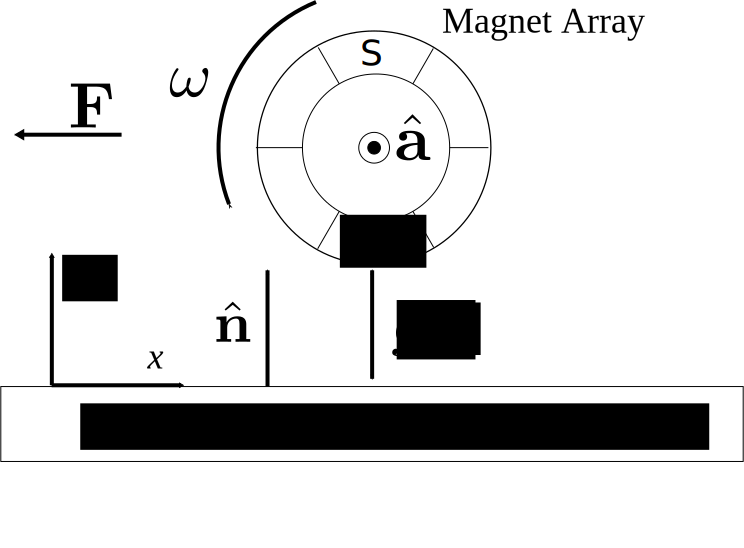
\includegraphics[width = 0.47\textwidth]{figures/spin_mag_diagram.eps}
      \caption{Inductance of oscillation winding on amorphous
       magnetic core versus DC bias magnetic field}
      \label{A single induction coupler}
   \end{figure}
   

Paudel and Bird derived an analytical solution for the force from a single rotating array of permanent magnets near a flat conductor. \cite{Paudel2013}

\begin{equation}
%\label{eq:Paudel55}
F^{ss} = \frac{w}{8\pi\mu_0} \int^{\infty}_{-\infty}\Gamma(\xi,g)|B^s(\xi,g)|^2 d\xi
\end{equation}
%equation explanation.
Where $\Gamma$ is a transmission function associated with the conductive surface and $B$ is the non-time-varying part of the array's magnetic field Fourier transformed with respect to $\hat{x}$.
% 
 $\Gamma$ and $B$ are nonlinear functions of the system state. $\Gamma$ depends on the array's rotation frequency $\omega$, velocity $\textbf{v}$ and distance from the surface $g$. $B$ is a nonlinear function of $g$ as well.  


\begin{equation}
\label{eq:arrayForce}
\textbf{F}_{PM} = A(g) \left(\textbf{a} \times \textbf{n} \right) \omega
\end{equation}



  
   

%
%The force on a conductive surface from a cyclic magnetic source 
%\begin{equation}
%\label{eq:sourcefield}
%B = B^s e^{i\omega t}
%\end{equation}
%is given by 
%\begin{equation}
%\label{eq:ForceInt}
%F^{ss} = \frac{w}{8\pi\mu_0}\int_{-\infty}^{\infty}\Gamma\left(\xi \right )\|B^s\left(\xi\right)\|d\xi
%\end{equation}
%here $B^s(\xi)$ is the Fourier transform of the static component of an oscillating source field  and $\Gamma(\xi)$ is a transmission function given in \cite{Paudel2013}. 
The upshot of this model is that a mechanically rotating array of permanent magnets will generate a force  force approximately perpendicular to the surface. 

\subsection{Permanent Magnets}
\subsection{Electromagnets}
\section{Movement Flavors}\label{sec:movements}
\subsection{Planar Movement}

   \begin{figure}[thpb]
      \centering
      %\framebox{\parbox{3in}{We suggest that you use a text box to insert a graphic (which is ideally a 300 dpi TIFF or EPS file, with all fonts embedded) because, in an document, this method is somewhat more stable than directly inserting a picture.}}

      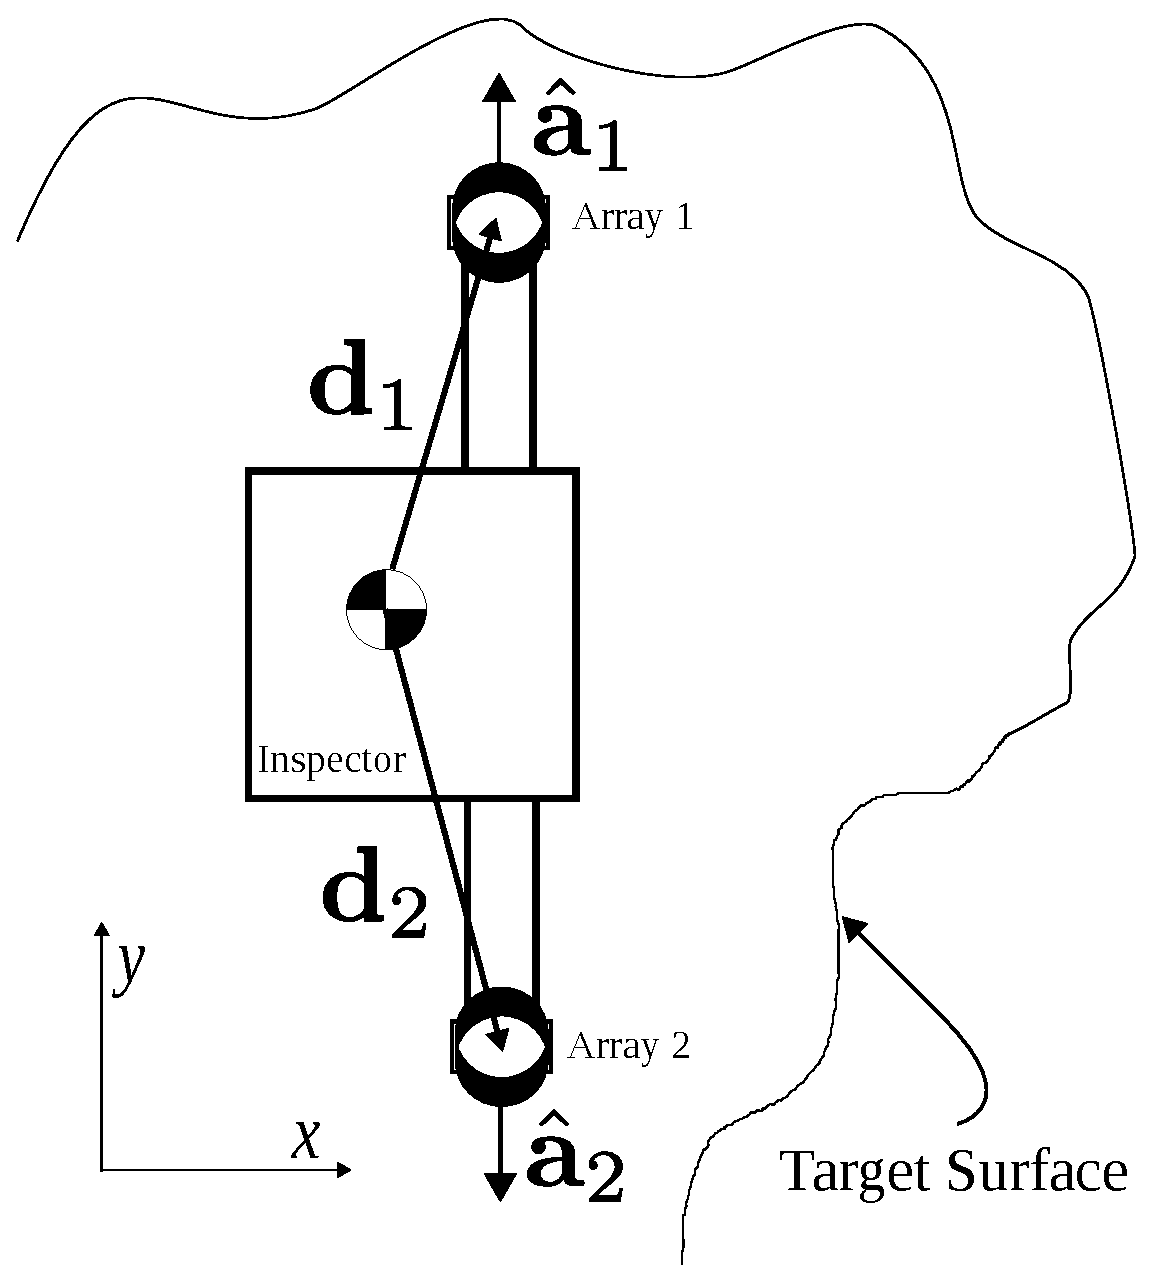
\includegraphics[width = 0.47\textwidth]{figures/surface_locomotion.eps}
      \caption{Inductance of oscillation winding on amorphous
       magnetic core versus DC bias magnetic field}
      \label{figurelabel}
   \end{figure}
   
   
     \begin{figure}[thpb]
      \centering
      %\framebox{\parbox{3in}{We suggest that you use a text box to insert a graphic (which is ideally a 300 dpi TIFF or EPS file, with all fonts embedded) because, in an document, this method is somewhat more stable than directly inserting a picture.}}

      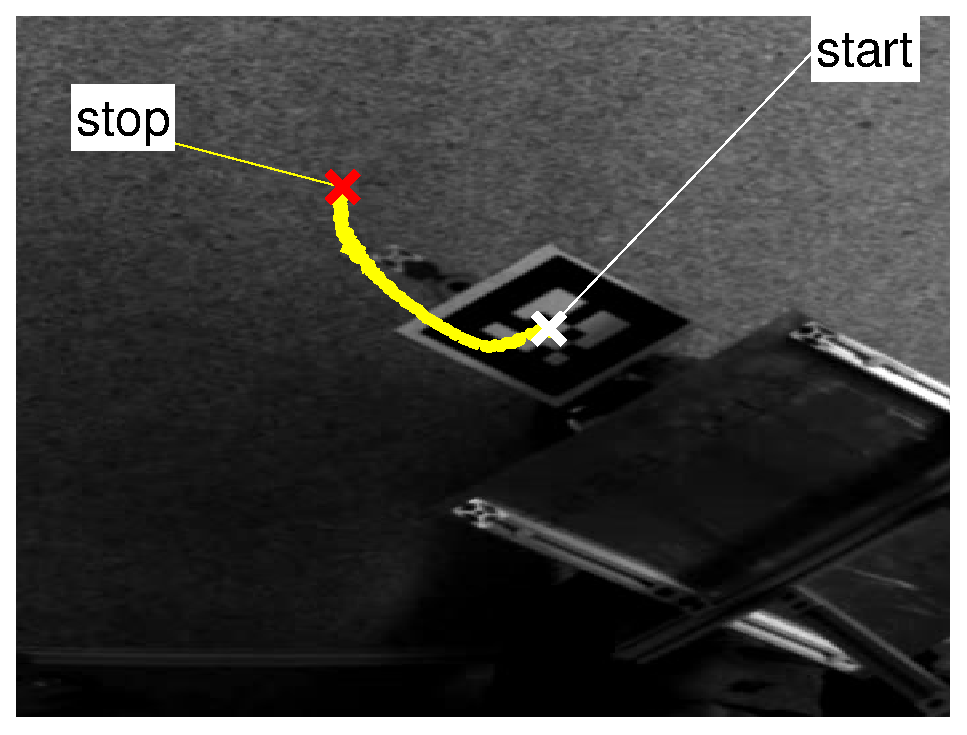
\includegraphics[width = 0.47\textwidth]{figures/planar_translation.eps}
      \caption{Inductance of oscillation winding on amorphous
       magnetic core versus DC bias magnetic field}
      \label{figurelabel}
   \end{figure}
   
      \begin{figure}[thpb]
      \centering
      %\framebox{\parbox{3in}{We suggest that you use a text box to insert a graphic (which is ideally a 300 dpi TIFF or EPS file, with all fonts embedded) because, in an document, this method is somewhat more stable than directly inserting a picture.}}

      \includegraphics[width = 0.47\textwidth]{figures/planar_rotations.eps}
      \caption{Inductance of oscillation winding on amorphous
       magnetic core versus DC bias magnetic field}
      \label{figurelabel}
   \end{figure}

%Define 'planar torque as torque perpendicular to the plane
%TODO Diagram
%TODO Pseudocode for algorithm 
\subsection{Out-of-Plane Movement}
%TODO Diagram

   \begin{figure}[thpb]
      \centering
      %\framebox{\parbox{3in}{We suggest that you use a text box to insert a graphic (which is ideally a 300 dpi TIFF or EPS file, with all fonts embedded) because, in an document, this method is somewhat more stable than directly inserting a picture.}}

      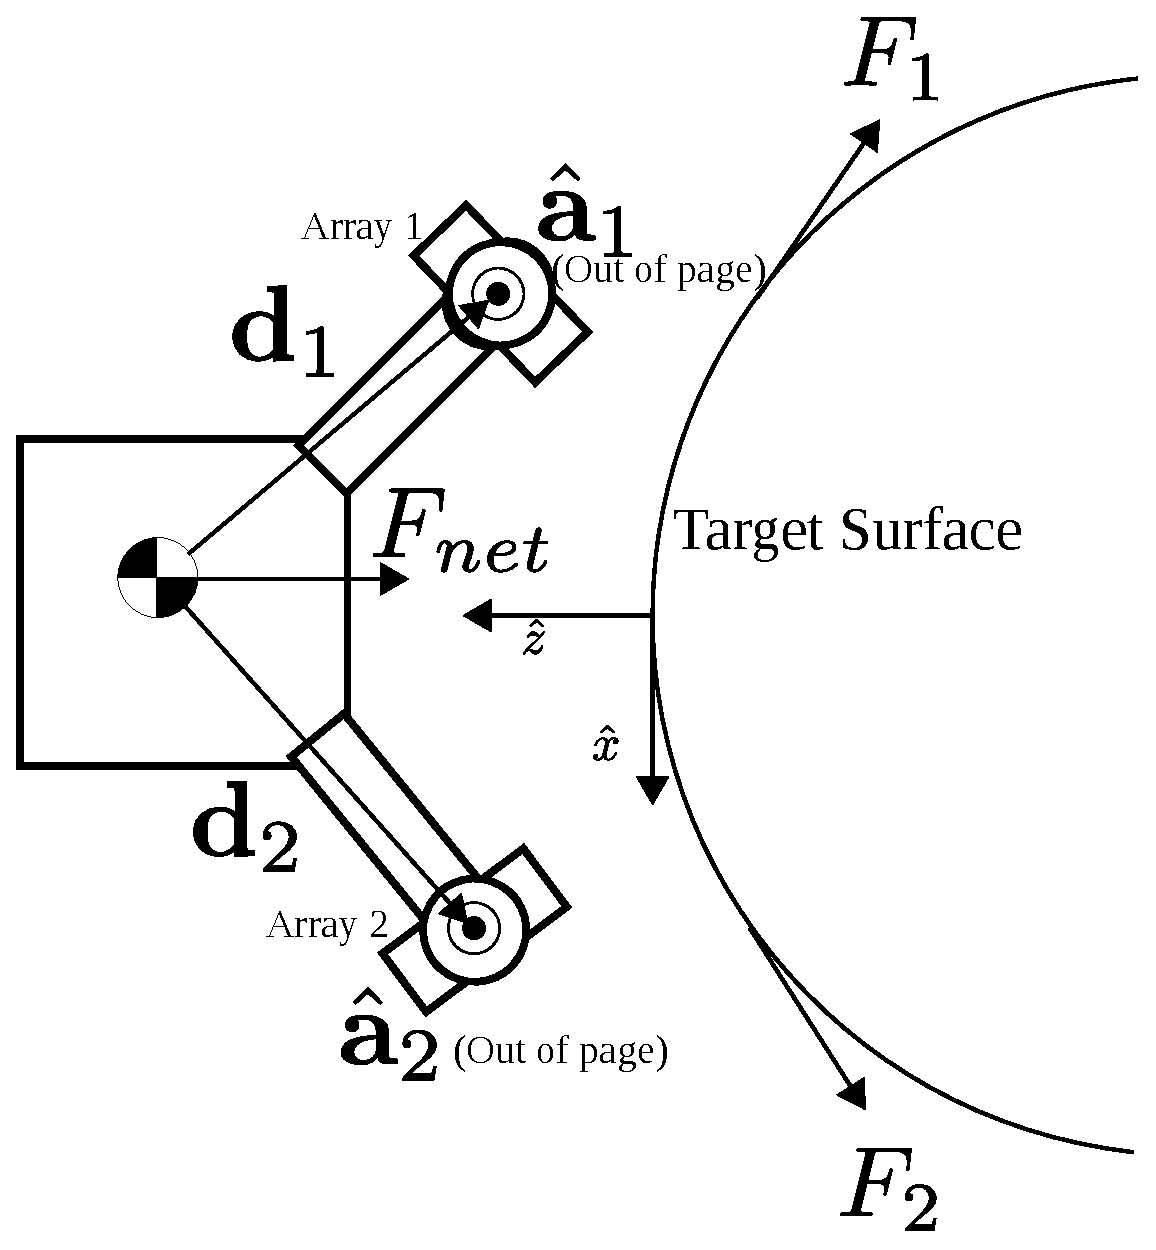
\includegraphics[width = 0.47\textwidth]{figures/curve_locomotion.eps}
      \caption{Inductance of oscillation winding on amorphous
       magnetic core versus DC bias magnetic field}
      \label{figurelabel}
   \end{figure}
%TODO Diagram

  \begin{figure}[thpb]
      \centering
      %\framebox{\parbox{3in}{We suggest that you use a text box to insert a graphic (which is ideally a 300 dpi TIFF or EPS file, with all fonts embedded) because, in an document, this method is somewhat more stable than directly inserting a picture.}}

      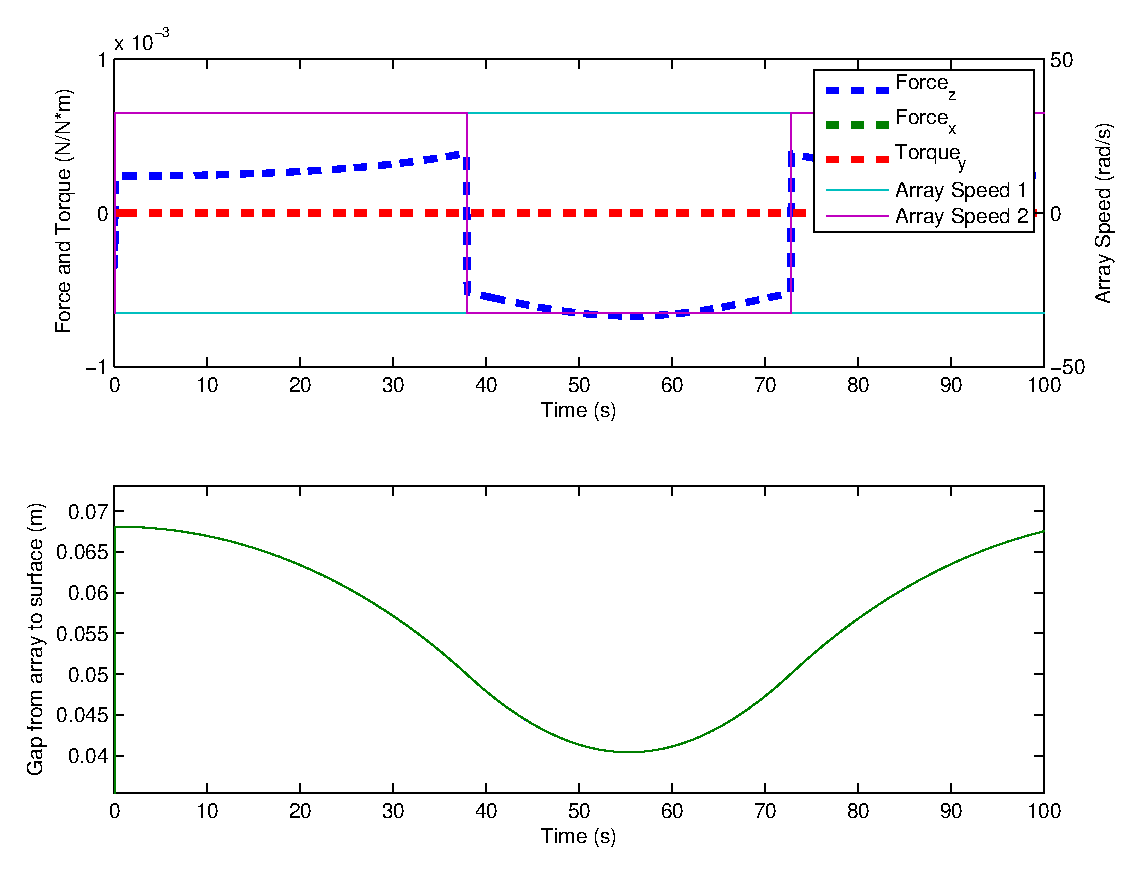
\includegraphics[width = 0.47\textwidth]{figures/curve_translations.eps}
      \caption{Inductance of oscillation winding on amorphous
       magnetic core versus DC bias magnetic field}
      \label{figurelabel}
   \end{figure}

   \begin{figure}[thpb]
      \centering
      %\framebox{\parbox{3in}{We suggest that you use a text box to insert a graphic (which is ideally a 300 dpi TIFF or EPS file, with all fonts embedded) because, in an document, this method is somewhat more stable than directly inserting a picture.}}

      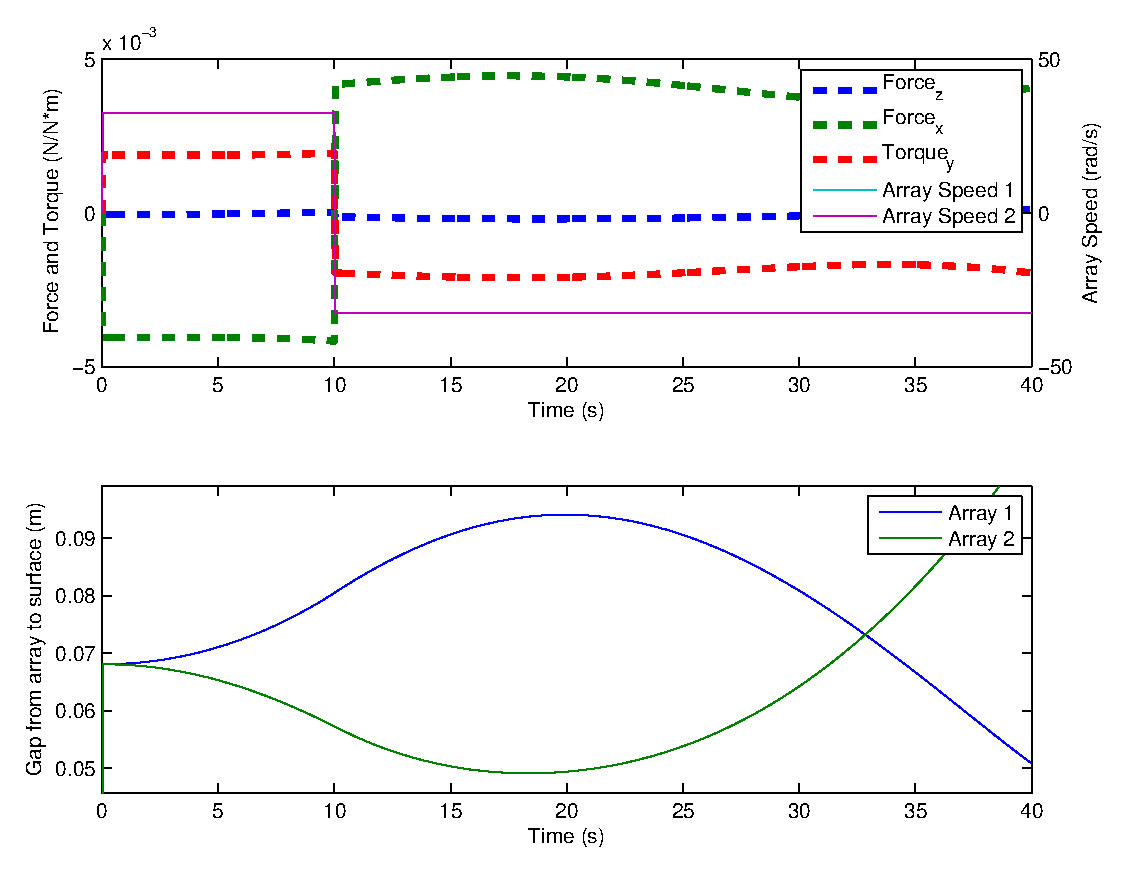
\includegraphics[width = 0.47\textwidth]{figures/curve_rotations.eps}
      \caption{Inductance of oscillation winding on amorphous
       magnetic core versus DC bias magnetic field}
      \label{figurelabel}
   \end{figure}


\section{Experimental Demonstration}\label{sec:experiments}
\section{Conclusion}
A robotic on-orbit service vehicle can use induction couplers can produce locomotive forces in all six rigid body degrees of freedom near a conductive surface. Rotating permanent-magnet arrays generate forces perpendicular to both their axes of rotation and the conductive surface. Current-oscillating electromagnets generate forces directly away from the surface. A pair of rotating arrays can produce $\hat{x}$ and $\hat{y}$ forces in the plane of the traversal surface. These two arrays can also produce torques in the $\hat{z}$ direction. This pair of arrays can take advantage of the surface geometry to generate forces in the $\hat{z}$ direction by generating shear forces along a non-flat surface whose $\hat{x}$ and $\hat{y}$ components cancel but whose $\hat{s}$ components add. A single electromagnet generates force in the $+\hat{z}$ direction. The force from the electromagnet can also generate torques based on its relative location to the system's center of mass. These maneuvers are demonstrated in simulations and verified on a low-friction testbed.  

%An autonomous space vehicle can use these forces to crawl over the conductive surface of a target spacecraft without propellant or the risk associated with physical grappling. Rotating arrays of magnets produce planar forces and torques. These rotating arrays can also produce forces perpendicular to the surface by taking advantage of surface features such as curvature or edges. Electromagnets can produce force directly away from any surface and by coupling these forces, produce torques parallel to that surface. Dynamic simulations demonstrate each degree-of-freedom using an analytical force model and hardware demonstrations on a low-friction testbed verify the results. 
%TODO future work - trajectory optimization, end effector design, kinematic simulation
Future work will focus on two areas - adaptive controllers and movement planning. A robotic inspector will need adaptive controllers to account for induction coupler's strong dependence on poorly known parameters of the environment.  The inspector will also need to plan movements carefully because its ability to exert control with an induction coupler is based on both its state, the local geometry.      

\begin{table}[h]
\caption{An Example of a Table}
\label{table_example}
\begin{center}
\begin{tabular}{|c||c|}
\hline
One & Two\\
\hline
Three & Four\\
\hline
\end{tabular}
\end{center}
\end{table}



   


\addtolength{\textheight}{-12cm}   % This command serves to balance the column lengths
                                  % on the last page of the document manually. It shortens
                                  % the textheight of the last page by a suitable amount.
                                  % This command does not take effect until the next page
                                  % so it should come on the page before the last. Make
                                  % sure that you do not shorten the textheight too much.

%%%%%%%%%%%%%%%%%%%%%%%%%%%%%%%%%%%%%%%%%%%%%%%%%%%%%%%%%%%%%%%%%%%%%%%%%%%%%%%%



%%%%%%%%%%%%%%%%%%%%%%%%%%%%%%%%%%%%%%%%%%%%%%%%%%%%%%%%%%%%%%%%%%%%%%%%%%%%%%%%



%%%%%%%%%%%%%%%%%%%%%%%%%%%%%%%%%%%%%%%%%%%%%%%%%%%%%%%%%%%%%%%%%%%%%%%%%%%%%%%%
\section*{APPENDIX}

\section*{ACKNOWLEDGMENT}




%%%%%%%%%%%%%%%%%%%%%%%%%%%%%%%%%%%%%%%%%%%%%%%%%%%%%%%%%%%%%%%%%%%%%%%%%%%%%%%%



\bibliography{icra_bib.bib}




\end{document}
